% 本文件是示例论文的一部分
% 论文的主文件位于上级目录的 `main.tex`

\chapter{粮食安全分析}
本章主要针对前两章由FRAR方法得到的各省影响作物产量最重要10位因素进行分析,进而对我国粮食生产及粮食安全提供建议。FRAR方法各省最重要因素如下表:

\begin{table}[!htbp]
    \centering
    \caption{FRAR:各省份最重要特征:1-5}
    \label{table:Feature5_FRAR1}
    \resizebox{\textwidth}{!}
    {
    \csvautobooktabular{data/ReducedFeatures_FRAR.csv}
    }
\end{table}
\setlength{\floatsep}{0pt}
\begin{table}[!htbp]
    \centering
    \caption{FRAR:各省份最重要特征:6-10}
    \label{table:Feature5_FRAR2}
    \resizebox{\textwidth}{!}
    {
    \csvautobooktabular{data/ReducedFeatures_FRAR2.csv}
    }
\end{table}

\section{结果分析}
本节主要从不同方面对玉米生产因素在全国各省的重要性进行比较,以便对我国粮食安全进行分析。

\subsection{化肥投入情况}
化肥一直是农业生产中影响作物产量的重要因素,不同作物根据自身所需的营养物质与土壤的不同也会对不同种类化肥有着不同的需求。\ref{fig:fertilizer_PN}展示了与化肥相关的属性中相对重要的磷肥与钾肥投入情况的重要度。
  \begin{figure}[htb]
    \centering
    \begin{minipage}[t]{0.49\linewidth}
      \centering
      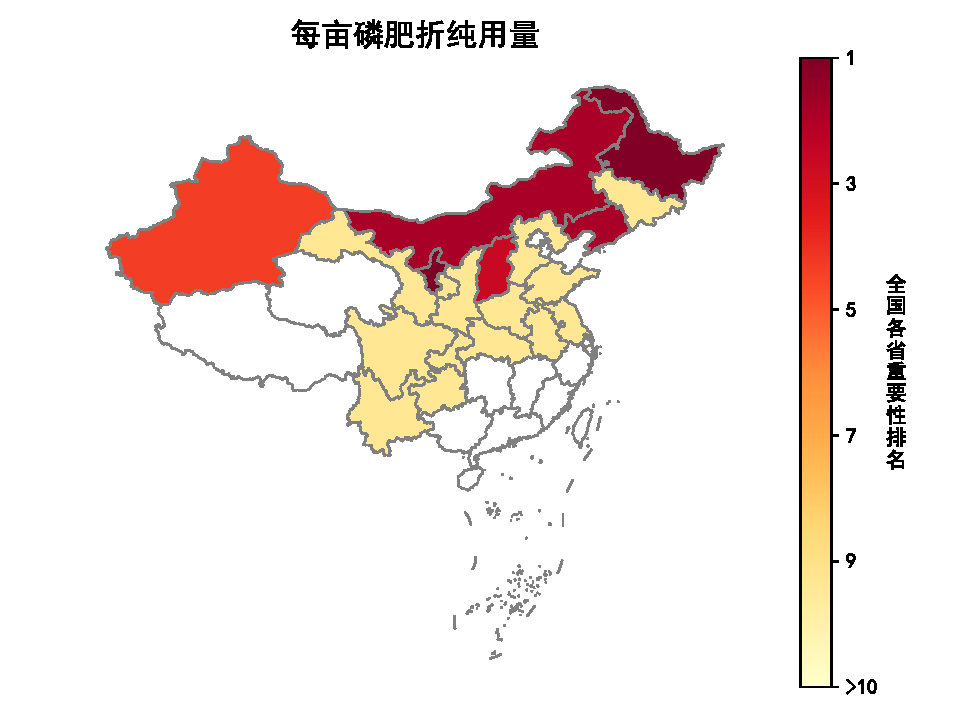
\includegraphics[width=\linewidth]{figs/NPK_P}
      \caption{磷肥}
      \label{fig:fertilizer_P}
    \end{minipage}
    \hfill
    \begin{minipage}[t]{0.49\linewidth}
      \centering
      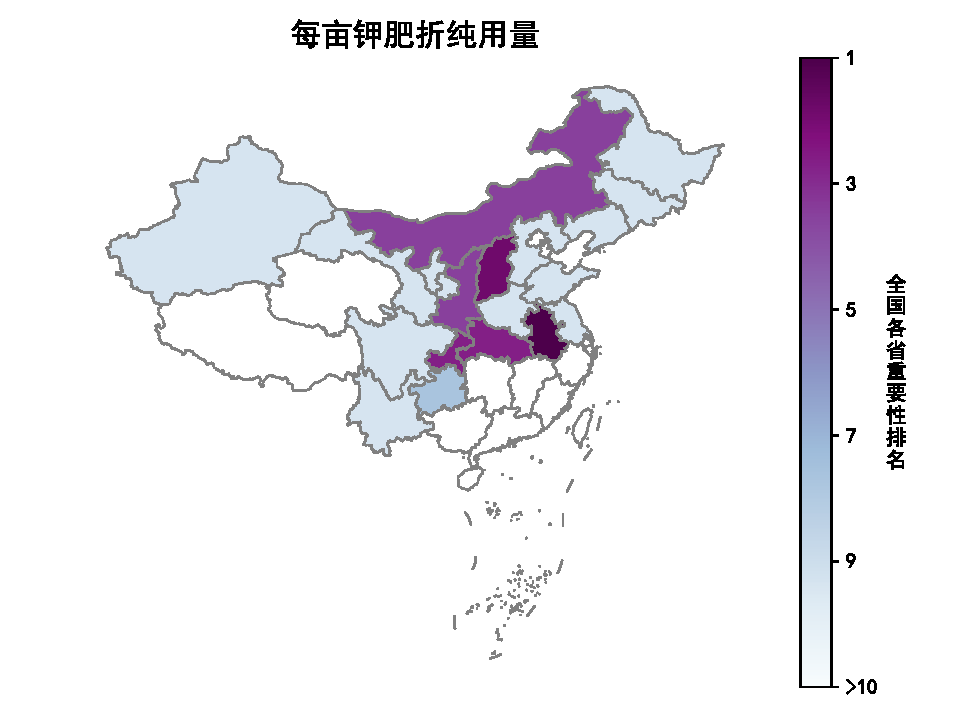
\includegraphics[width=\linewidth]{figs/NPK_K}
      \caption{钾肥}
      \label{fig:fertilizer_K}
    \end{minipage}
    \caption{每亩磷肥与钾肥折纯用量}
    \label{fig:fertilizer_PN}
  \end{figure}

从图中可以看出,磷肥与钾肥主要对个别集中的省份的影响较大。磷肥主要对东北省份及内蒙古、宁夏、山西影响较大,这可能与我国北方土地缺磷有关。钾肥主要对我国安徽、湖北、重庆等中南部地区及山西、陕西、内蒙古等北部省份影响较大。其中,磷肥与钾肥同时对内蒙古和山西玉米产量影响较大。

磷肥与钾肥对玉米产量的影响不同。玉米施用磷素化肥,穗粒数有明显增加。玉米施用钾素化肥增产的主要表现是提高百粒重,增加穗粒数\cite{施用氮磷钾肥对夏玉米产量和品质的影响}。磷肥的施入能够有效提升玉米产量,增加玉米种植经济效益,但过量施入磷肥会导致玉米产量及经济效益降低\cite{磷肥用量对玉米产量的影响}。因此在农业生产中应合理配施磷、钾肥, 促进养分比例的协调供给和保持养分平衡, 使玉米对磷、钾营养元素的吸收增多\cite{磷钾肥配合施用对玉米产量及养分吸收的影响}。在农业生产实践中,不同省份要根据其特定的土壤性质与气候条件,调整合理的磷钾肥使用量。而俄乌两国作为农作物肥料的主要供应国,占全球化肥出口贸易总额的近四分之一。在俄乌冲突导致全球化肥供应紧张的情况下,还应尽量保障图中磷钾肥对玉米生产较为重要的省份的供应充足,以此保障我国粮食生产与安全。


% \subsection{化肥投入情况}
% 化肥一直是农业生产中影响作物产量的重要因素,不同作物根据自身所需的营养物质与土壤的不同也会对不同种类化肥有着不同的需求。下面\ref{fig:fertilizer_PN}是磷肥与钾肥投入情况的重要度。
%   \begin{figure}[htb]
%     \centering
%     \begin{minipage}[t]{0.49\linewidth}
%       \centering
%       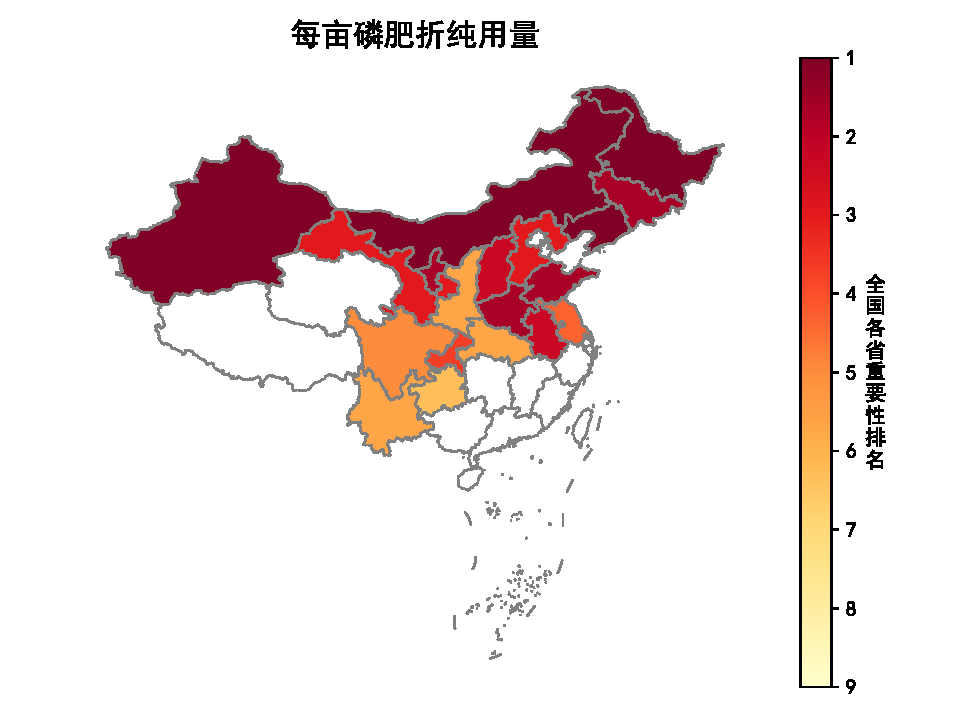
\includegraphics[width=\linewidth]{figs/fertilizer_P.pdf}
%       \caption{磷肥}
%       \label{fig:fertilizer_P}
%     \end{minipage}
%     \hfill
%     \begin{minipage}[t]{0.49\linewidth}
%       \centering
%       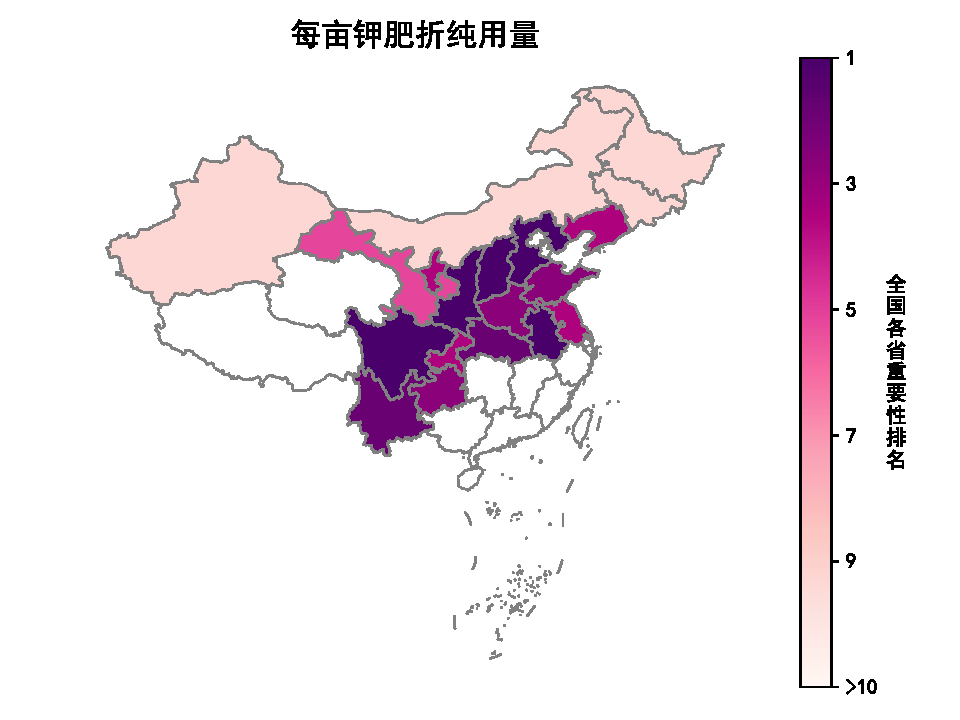
\includegraphics[width=\linewidth]{figs/fertilizer_K.pdf}
%       \caption{钾肥}
%       \label{fig:fertilizer_K}
%     \end{minipage}
%     \caption{每亩磷肥与钾肥折纯用量}
%     \label{fig:fertilizer_PN}
%   \end{figure}

% 从图中可以看出,钾肥与磷肥是影响玉米亩产的重要因素,其中磷肥在我国北方省份的重要程度集中在前3,钾肥在我国南方省份也有着相同的重要程度。而我国由于纬度跨度大地形复杂,南北方土壤的土壤肥力与营养元素含量也有着较大差异,图中结果恰好与我国北方土壤缺磷南方缺钾相应,也从侧面说明了本文实验结果的正确性。

% 图中结果显示在我国19个省份中磷肥钾肥在16个省份中占据了前三名的位置,说明磷肥钾肥在玉米生长过程中起着至关重要的作用,且南北方对两种化肥的需求不同,北方对磷肥需求大而南方对钾肥需求大,在农业生产实践中,南北方不同省份要根据其特定的土壤性质与气候条件,调整合理的磷钾肥使用量。而俄乌两国作为农作物肥料的主要供应国,占全球化肥出口贸易总额的近四分之一。在俄乌冲突导致全球化肥供应紧张的情况下,还应尽量保障北方磷肥与南方钾肥的供应充足,以此来保障我国粮食生产与安全。

% 本文实验数据中除了磷肥钾肥外,还包含了氮肥、复混肥、农家肥,其中\ref{fig:fertilizer_NF}展示了氮肥与农家肥投入情况的重要程度。

% \begin{figure}[htb]
%   \centering
%   \begin{minipage}[t]{0.49\linewidth}
%     \centering
%     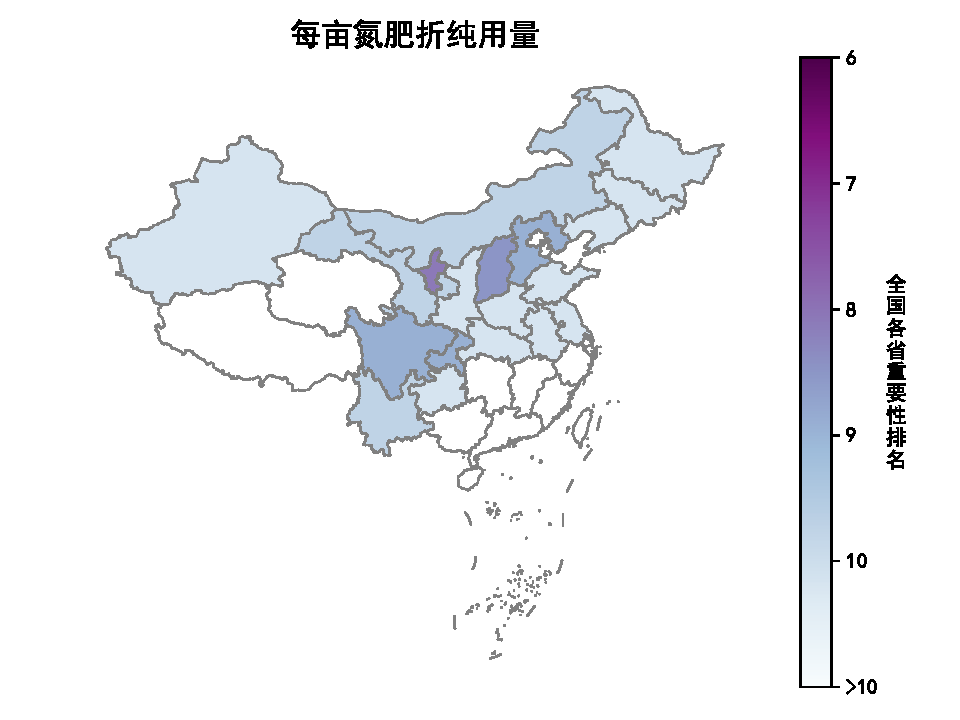
\includegraphics[width=\linewidth]{figs/fertilizer_N.pdf}
%     \caption{氮肥}
%     \label{fig:fertilizer_N}
%   \end{minipage}
%   \hfill
%   \begin{minipage}[t]{0.49\linewidth}
%     \centering
%     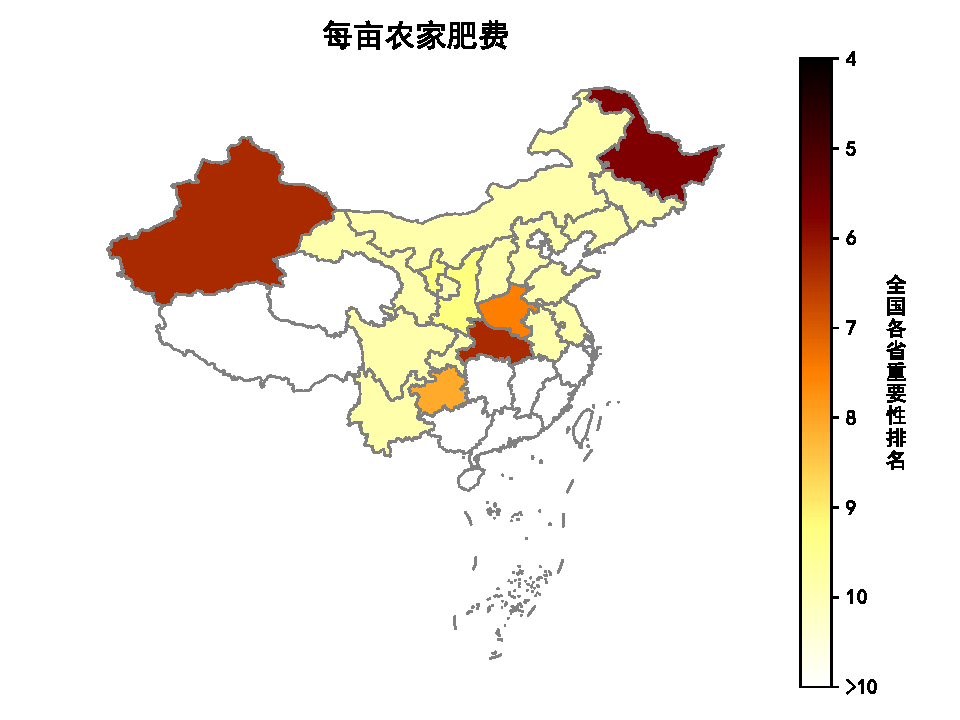
\includegraphics[width=\linewidth]{figs/fertilizer_farmyard.pdf}
%     \caption{农家肥}
%     \label{fig:fertilizer_farmyard}
%   \end{minipage}
%   \caption{每亩氮肥与农家肥折纯用量}
%   \label{fig:fertilizer_NF}

% \end{figure}

% 从图中可以看出,与磷肥钾肥大都集中在重要性前三不同,氮肥在全国重要性大都集中在第10名及以外,这可能是在大多数情况下,我国氮肥水平已经很高了,土壤中的氮素含量已经足够满足玉米生长的需要,过量的氮肥可能会对作物生长产生负面影响,因此氮肥对玉米产量的影响不大,在生产过程中注意适量施用氮肥。\cite{刘明鹏2022氮肥施用对四川紫色土矿质态氮淋失特征及春玉米产量的影响}然而复混肥作为一种混合肥料,其基本功能可以由其余氮磷钾肥相抵,在基本上所有省份中都没有进入重要性前10,对玉米产量并没有特别显著的影响。

% 而农家肥作为有机肥的一种,在实现有机农业、保护土地等方面有着重要的作用,其中以黑龙江黑土地为代表,其在自然条件下富含有机质且肥力高,而长期过度耕作和不合理的施肥方式都会导致土壤质量下降,因此保护黑土地非常重要。对于黑土地的管理和保护需要采取合理的耕作措施和施肥方案,充分利用农家肥等有机肥料可以保持土壤肥力和生产力的稳定,且农家肥在保护黑土地的同时,还能帮助农户节本增效。同理新疆因气候地理原因土地养分相对较少,施用农家肥可提高土地肥力改善土壤结构。因而在黑龙江、新疆等个别省份在农耕中要格外重视农家肥的影响。

% 因此建议农民在施用肥料时,做到因地制宜,根据当地土壤质量和作物需求的不同,适量施用农家肥,达到肥料的最佳配比,提高农业生产的效益和可持续性。

% \subsection{自然灾害}

% \begin{figure}[htb]
%   \centering
%   \begin{minipage}[t]{0.49\linewidth}
%     \centering
%     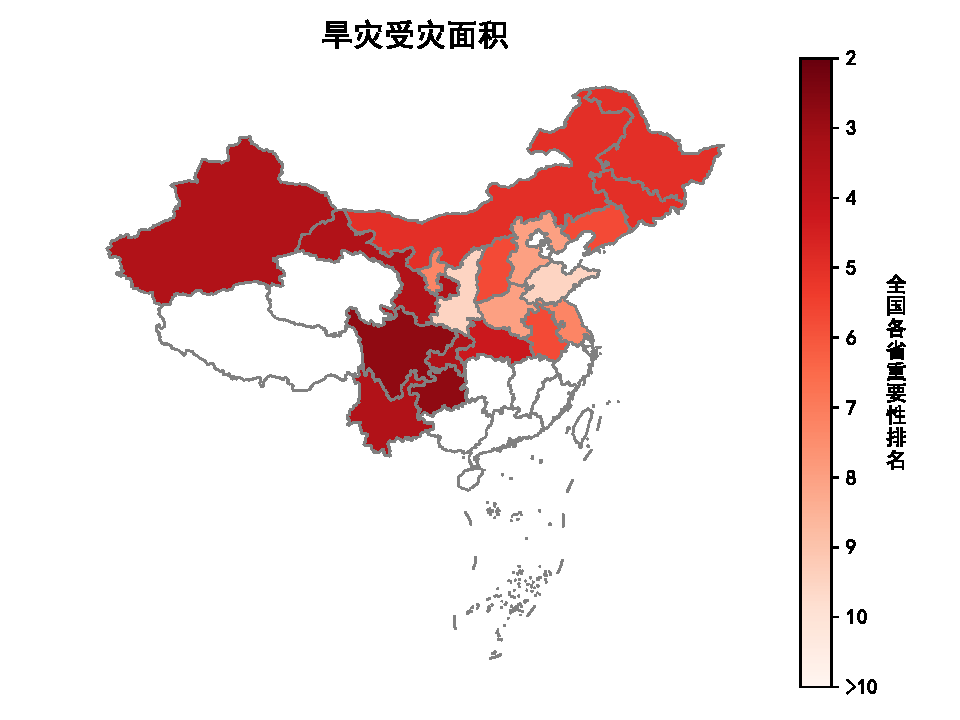
\includegraphics[width=\linewidth]{figs/hazard_drought.pdf}
%     \caption{旱灾}
%     \label{fig:hazard_drought}
%   \end{minipage}
%   \hfill
%   \begin{minipage}[t]{0.49\linewidth}
%     \centering
%     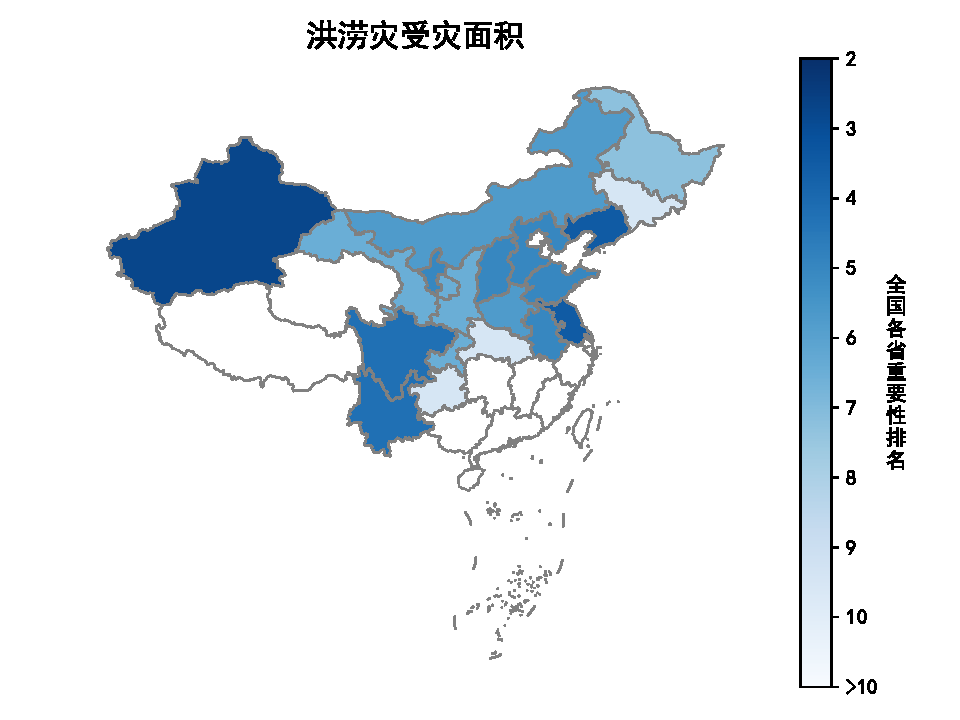
\includegraphics[width=\linewidth]{figs/hazard_flood.pdf}
%     \caption{洪涝灾}
%     \label{fig:hazard_flood}
%   \end{minipage}
%   \caption{旱灾与洪涝受灾面积}
%   \label{fig:hazard}
% \end{figure}

% 自然灾害作为影响作物生长的直接因素,直接影响着受灾地区作物的生长与丰收。而旱灾与洪涝灾害作为最常见的灾害,分析其主要影响区域对于作物种植有着重要意义。\ref{fig:hazard}展示了全国各省旱灾洪灾影响因子的重要性排名。

% 图中结果展示了我国旱灾与洪涝灾害对玉米产量有着非常大的影响,在近一半省份中均排在了重要性前5。其中中国西部的西南农业区受旱灾影响最严重,例如四川、贵州、新疆等地的常年遭遇旱灾,对当地农作物的生长有着较大的影响。此外,我国新疆、西南地区及辽宁江苏等沿海省份受到洪涝灾害影响也较严重,对玉米的生长及产量有着较大的影响。

% 其中四川、云南位于中国西南地区,虽属于亚热带季风气候区域,但由于受到地形和气候的影响,这些地区的降雨量和水资源分布非常不均衡,同时也对排灌设施的建设和维护带来了较大困难,造成了干旱和水灾等自然灾害的频繁发生。对于新疆而言,其地理位置位于亚欧大陆腹地,是典型的内陆干旱地区,旱灾频繁发生,但因其三山夹两盆的特殊地形和独特的自然环境格局,同时较容易受到洪涝灾害的严重影响。\cite{哈斯也提·热合曼2020新疆}

% 对于新疆、四川、云南等省份而言,两种灾害对玉米产量的影响因素基本全排在重要性前4位,说明这两种自然灾害作为影响玉米生产的重要因素,已经对其产量产生了较为严重的负面影响。因此对于容易受到旱灾影响的省份,应加强土地的水分管理,提高灌溉效率,减少土地退化和干旱损失。对于容易受到洪涝灾害影响的省份,建议加强防洪和排灌设施的建设,提高其应急响应能力。因在不同省份旱灾和洪涝灾害对玉米产量的影响各不相同,各省份应根据其本身的气候特点和土地条件,采取相应的防范措施。

\subsection{成本投入情况}
\begin{figure}[htb]
  \centering
  \begin{minipage}[t]{0.49\linewidth}
    \centering
    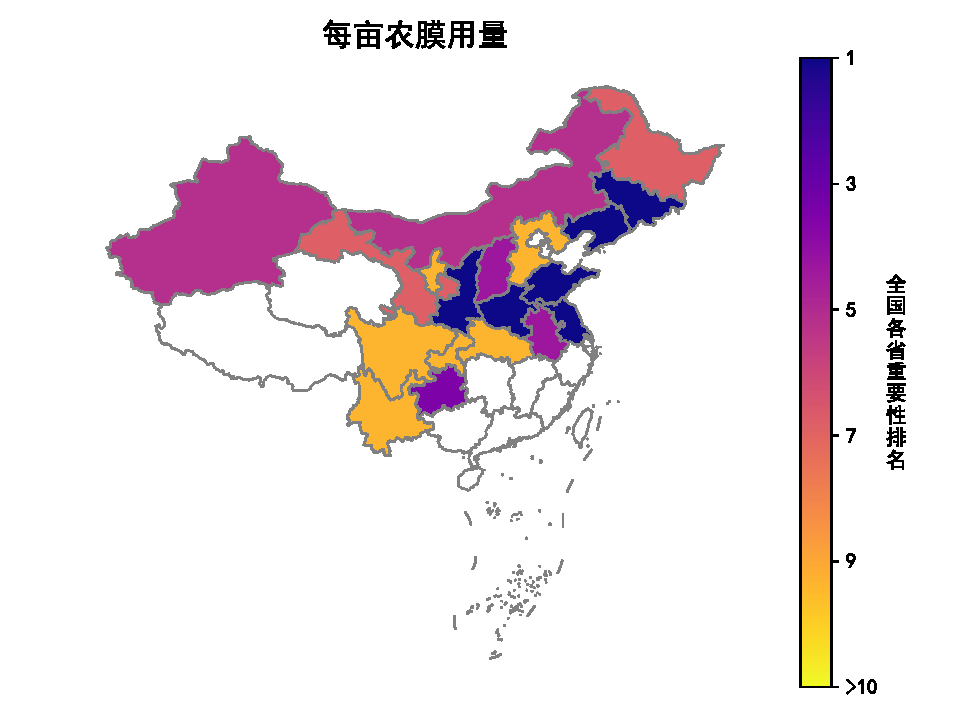
\includegraphics[width=\linewidth]{figs/InputCost_Film}
    \caption{农膜投入}
    \label{fig:InputCost_Film}
  \end{minipage}
  \hfill
  \begin{minipage}[t]{0.49\linewidth}
    \centering
    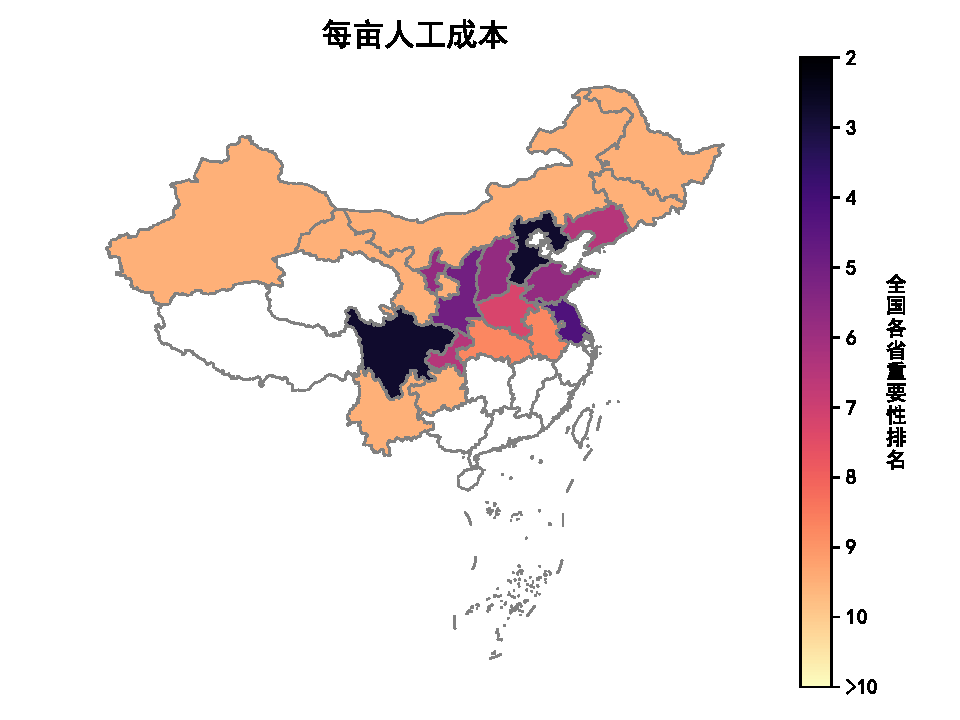
\includegraphics[width=\linewidth]{figs/InputCost_Labor}
    \caption{人工成本}
    \label{fig:InputCost_Labor}
  \end{minipage}
  \caption{成本投入情况}
  \label{fig:input_FL}
\end{figure}

在成本投入情况中,每亩农膜用量与每亩人工成本对玉米产量有着较为重要的影响。因此\ref{fig:input_FL}中展示了这两个变量的重要程度。

20世纪80年代初我国开始应用农作物地膜覆盖技术,地膜覆盖技术可以起到增温保湿作用, 使农作物增产的同时也提高了农产品品质, 为社会带来巨大的经济效益。然而过多的农膜残留在土壤中也增加了清膜成本, 同时又会破坏土壤结构\cite{可降解农膜在玉米上的应用研究}。因此对于每亩农膜用量而言,收成并不一定与用量成正比。如果每亩农膜用量过多,会导致土壤过于密封,通气性差,不利于农作物的根系呼吸,容易发生病虫害,且会阻碍水分和养分的渗透,影响农作物的吸收和利用,同时不可降解农膜还会破坏土壤结构造成环境污染。而如果每亩农膜用量过少,会无法达到良好的保温、保湿、杀菌和抗旱效果,容易导致农作物受到干旱和低温等自然灾害的影响,产量和质量也会受到影响。由\ref{fig:InputCost_Film}可得,我国陕西、河南、内蒙古、新疆等中西部省份可能由于土壤、气候等因素导致水分养分蒸发流失较快,因而适量增加农膜使用可以保持水分、养分和温度。而吉林、辽宁、山东、江苏等东北及沿海地区由于气候湿度等原因,使用农膜可以一定程度上保持温度与湿度,进而提高产量。因而在沿海地区与中西部地区在玉米种植过程中要注意合理使用农膜。

每亩人工成本代表的是农业生产中的劳动力市场情况与农业机械化程度。一般来说每亩人工成本的重要性越高,意味着该地区玉米生产对于人工劳动力的依赖程度越高,农业机械化程度较低,同时说明农业劳动力市场较为匮乏。由\ref{fig:InputCost_Labor}可得,每亩人工成本对四川、河北玉米产量有着很大的影响,对陕西、山东、江苏等中部及沿海省份也有着较大的影响,这与发达省份人工劳动力成本高及农业机械化程度均有关。因而对于劳动力市场人工成本较高的省份应注意提高农业机械化的建设与发展,减少对人工劳动力的依赖;对于地形复杂耕作成本较高的地区,可以通过提高农业机械化水平与加大人工劳动力投入来提高玉米产量。

% \subsection{物化投入情况}
% \begin{figure}[htb]
%   \centering
%   \begin{minipage}[t]{0.49\linewidth}
%     \centering
%     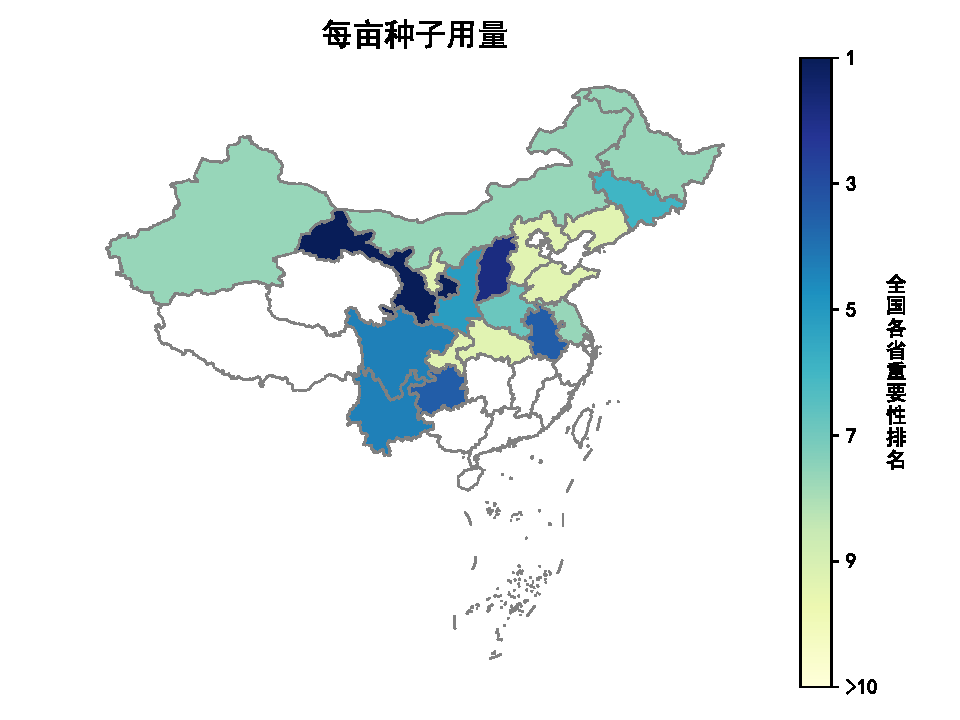
\includegraphics[width=\linewidth]{figs/input_Seeds.pdf}
%     \caption{种子}
%     \label{fig:input_Seeds}
%   \end{minipage}
%   \hfill
%   \begin{minipage}[t]{0.49\linewidth}
%     \centering
%     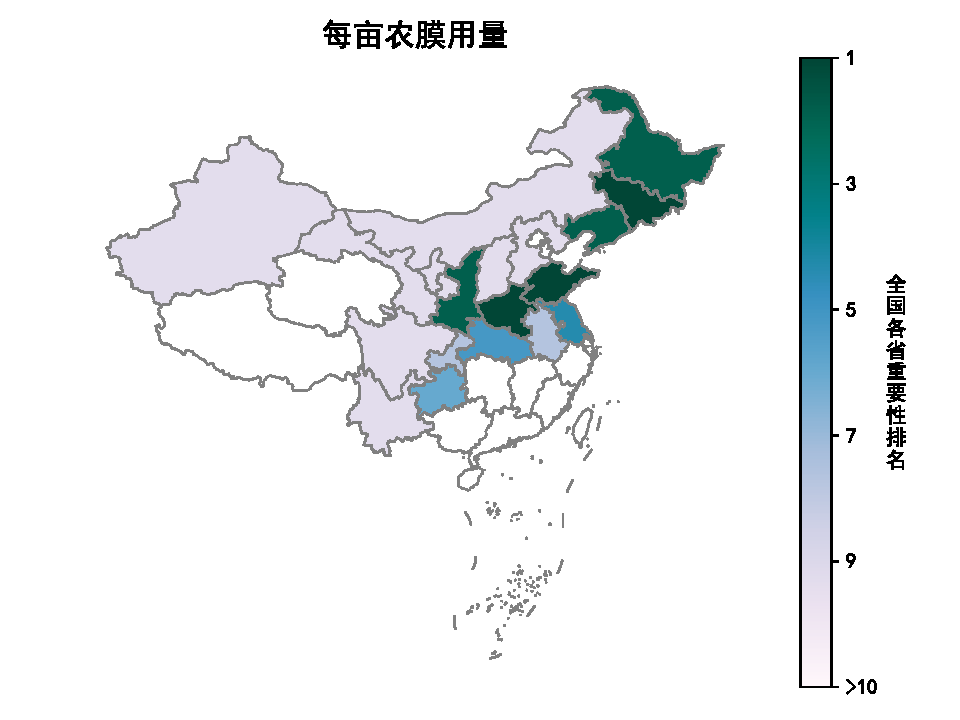
\includegraphics[width=\linewidth]{figs/input_AgriFilm.pdf}
%     \caption{农膜}
%     \label{fig:input_AgriFilm}
%   \end{minipage}
%   \caption{物化投入情况}
%   \label{fig:input_AS}
% \end{figure}

% 在物化投入情况中,仅有每亩种子用量和每亩农膜用量这两个变量在全国各省中具有较为重要的排名。因此\ref{fig:input_AS}中展示了这两个变量的重要程度。而解释变量玉米播种面积在各省重要性排名中均为进入前10,恰好印证了玉米的亩产与播种面积无关。


% 对于每亩种子用量来说,其收成与用量并不是成正比。如果每亩种子用量过多,会导致种植密度过高,单株营养面积小,影响作物之间的空间竞争,从而降低产量和质量,且造成种子浪费增加农民成本。如果种子用量过少,每亩土地难以保证应有的苗数,降低产量的同时还会降低土地利用效率。因而由\ref{fig:input_Seeds}可得甘肃、山西、贵州等中西部地区在玉米种植过程中要进行合理密植,科学选择每亩种子用量。\cite{董云2015填充物与用种量对机械化条播油菜群体质量及产量的影响}


% 对于每亩农膜用量而言,收成也并不一定与用量成正比。如果每亩农膜用量过多,会导致土壤过于密封,通气性差,不利于农作物的根系呼吸,容易发生病虫害,且会阻碍水分和养分的渗透,影响农作物的吸收和利用,同时还会造成环境污染。而如果每亩农膜用量过少,会无法达到良好的保温、保湿、杀菌和抗旱效果,容易导致农作物受到干旱和低温等自然灾害的影响,产量和质量也会受到影响。由\ref{fig:input_AgriFilm}可得,山东、河南、陕西等地区可能由于土壤、气候等因素导致水分养分蒸发流失较快,因而适量增加农膜使用可以保持水分、养分和温度。而东北三省地区较为寒冷,使用农膜可以一定程度上提高土壤温度,进而提高产量。因而在东北三省地区与中原地区在玉米种植过程中要注意合理使用农膜。

\subsection{排灌建设情况}

\begin{figure}[htb]
    \centering
    \begin{minipage}[t]{0.49\linewidth}
      \centering
      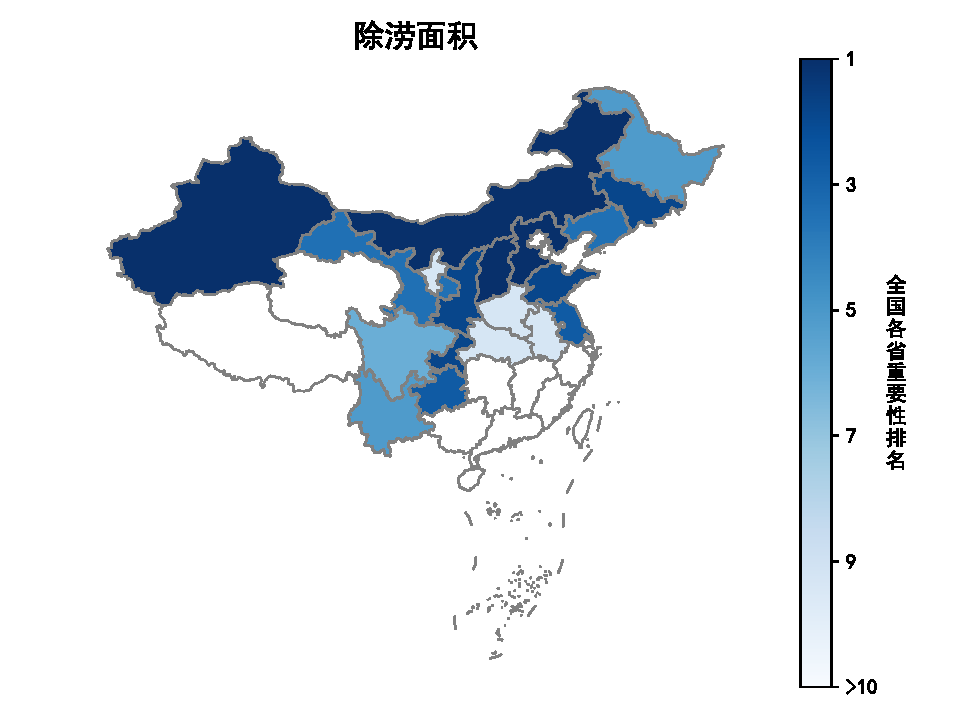
\includegraphics[width=\linewidth]{figs/DrainIrrigate_WaterLogging}
      \caption{除涝面积}
      \label{fig:DrainIrrigate_WaterLogging}
    \end{minipage}
    \hfill
    \begin{minipage}[t]{0.49\linewidth}
      \centering
      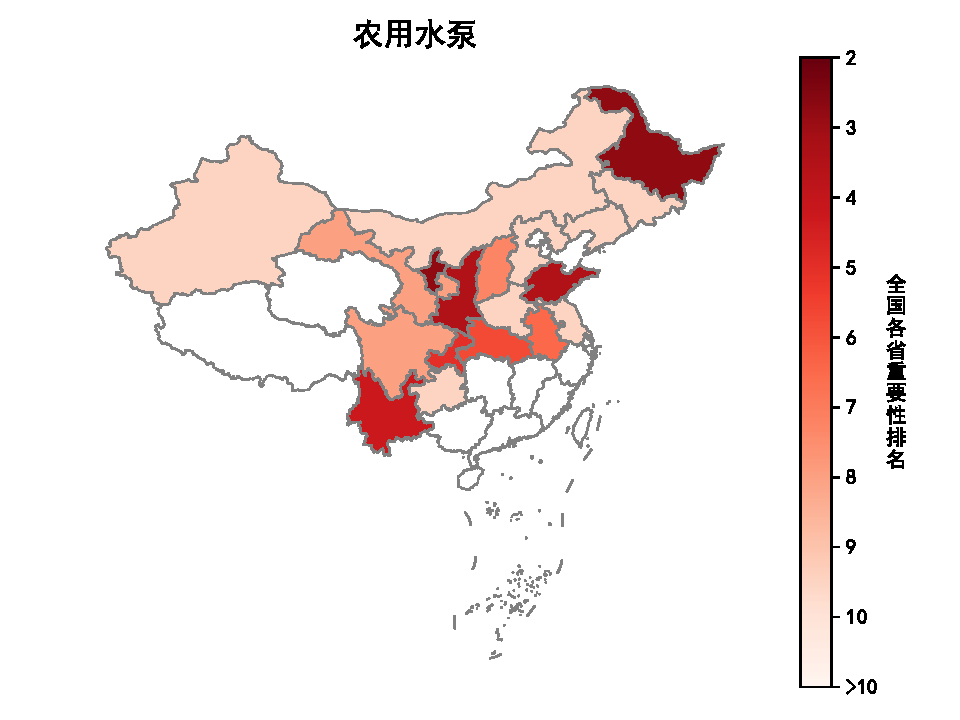
\includegraphics[width=\linewidth]{figs/DrainIrrigate_WaterPump}
      \caption{农用水泵}
      \label{fig:DrainIrrigate_WaterPump}
    \end{minipage}
    \caption{排灌建设情况}
    \label{fig:DrainIrrigate}
  \end{figure}

  在排灌建设情况中,除涝面积代表着排水情况,农用水泵数代表着灌溉情况,因此\ref{fig:DrainIrrigate}中展示了这两个变量的重要程度。

  \ref{fig:DrainIrrigate_WaterLogging}显示除涝面积对于我国新疆、内蒙古、山西、河北等中西部省份及部分沿海省份的玉米生产影响较大,除涝面积的大小对于保护和维持玉米生产的稳定性具有重要作用,增加除涝面积可以减少因洪涝灾害而导致的玉米受灾面积和产量损失。对于受到除涝面积影响大的省份,说明雨涝洪涝在这些省份对于玉米的生长产生了较大的影响,因而在生产过程中格外注意在雨涝洪涝后及时开展除涝补救措施,以减少因雨涝导致的玉米减产\cite{东北三省地区生长季旱涝对春玉米产量的影响}。
  
  而\ref{fig:DrainIrrigate_WaterPump}显示农用水泵对于我国黑龙江、宁夏、陕西、云南、山东等个别省份的玉米生产有较大的影响。农用水泵反映着农业生产中的灌溉水平与规模,对于农用水泵在玉米生产中有着较高重要度的省份,说明该地区因气候环境土壤等原因导致玉米生长对于灌溉设施有着较大的依赖,在玉米生产中这些地区要格外重视灌溉设施的建设与完善,加强灌溉设施的投入力度,优化农田水利设施建设,提高灌溉效率和节水利用,并在旱季加大对玉米的灌溉力度,避免因灌溉不足而导致的减产发生。

  根据排灌建设情况对不同省份玉米产量的影响,可以得出水分对玉米生长有着重要的影响。对于受到影响较大的省份,政府应该加大对这些地区的排灌设施建设和维护力度,提高排灌设施的效率与覆盖面积。对于受到排灌费影响较小的地区,也应加强设施的完善与维护,同时应鼓励农民使用节水灌溉技术,尽可能降低排灌成本与节约用水量。

  \subsection{机械化建设情况}
  \begin{figure}[htb]
      \centering
      \begin{minipage}[t]{0.49\linewidth}
        \centering
        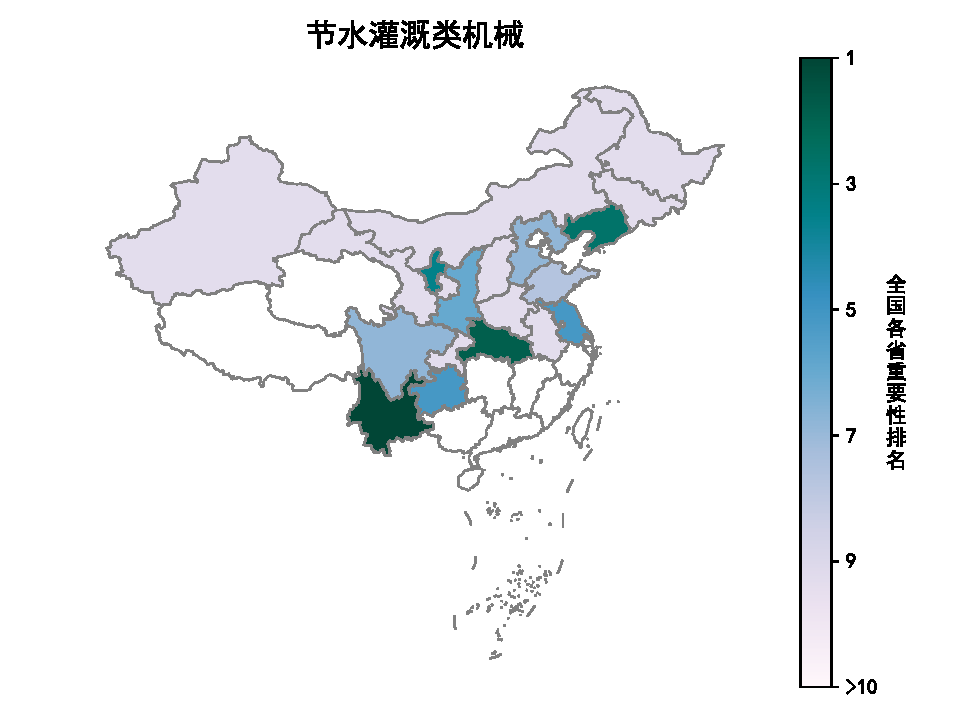
\includegraphics[width=\linewidth]{figs/Mechanization_IrrigationMachinery}
        \caption{灌溉机械}
        \label{fig:Mechanization_IrrigationMachinery}
      \end{minipage}
      \hfill
      \begin{minipage}[t]{0.49\linewidth}
        \centering
        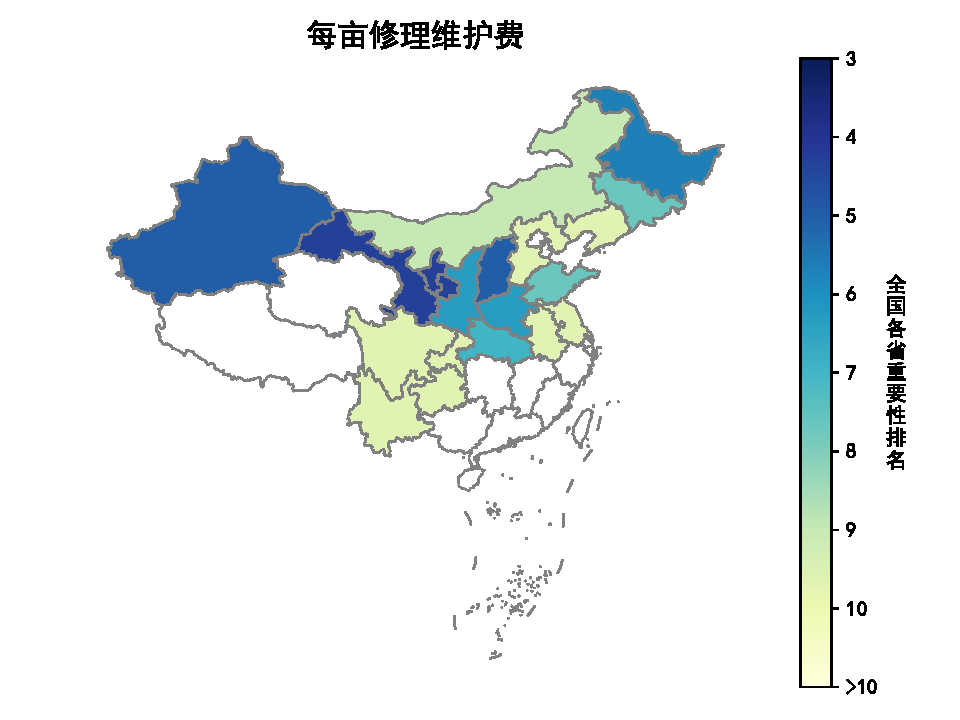
\includegraphics[width=\linewidth]{figs/Mechanization_Repair}
        \caption{修理维护}
        \label{fig:Mechanization_Repair}
      \end{minipage}
      \caption{机械化建设情况}
      \label{fig:Mechanization}
    \end{figure}

在机械化建设情况中,一个地区农用机械拥有量可以反映其农业机械化发展程度。节水灌溉类机械作为农业机械中关键的一部分,是指在农业生产中用于提高灌溉效率、减少用水量的设备和工具。一个地区节水灌溉类机械持有量越多代表着该地区农业灌溉机械化与自动化越发达。每亩修理维护费主要反映了农业机械设备的使用情况和维护保养水平。如果农业机械设备使用频率高、年限长、维护保养不及时,就会导致每亩修理维护费增加。因此节水灌溉机械持有量可以反映某地区机械化的体量与发展程度,而每亩修理维护费可以反映某地区灌溉机械的设备可靠性、生产稳定性及灌溉效率与成本。研究表明我国玉米灌溉属国际较低水平,水分对玉米的生长起着至关重要的作用,是影响玉米最终产量的重要因素,因此, 在进行玉米灌溉时应尽量选择灌溉效果较好的方式进行作业, 节水灌溉机械化播种作业技术就是一种提升玉米出苗率、玉米产量的有效方法\cite{浅谈玉米节水灌溉机械化播种作业技术}。

对于节水灌溉类机械,如\ref{fig:Mechanization_IrrigationMachinery}中结果所示,其对我国云南、湖北、宁夏、辽宁等省份的玉米产量有着较大影响,针对地形复杂与发展相对落后的地区,加强节水灌溉设施建设将有助于提高农业机械化程度,进而显著提高生产效率。针对气候干旱的地区,由于水分对玉米的生长有着重要的作用,因此加大节水灌溉机械的建设力度能够在旱季中保持玉米生长的水分需求,避免了因干旱导致的减产。

对于每亩修理维护费,由\ref{fig:Mechanization_Repair}可以看出,每亩修理维护费对我国甘肃、宁夏、新疆、山西、黑龙江等省份的玉米生产影响较大。每亩修理维护费相较于节水灌溉类机械,可以反映生产设备的质量、维护管理的水平及生产环境的条件。针对这些对玉米生产影响较大的省份,在购买农业机械设备时优先选择质量可靠、耐用性好的设备,并加强农业机械设备的维护管理工作,定期进行检查和保养,同时改善农田环境条件,以减少机械设备在作业过程中的损耗和故障风险。通过减少农业生产中的农业机械的损耗,有助于降低修理维护费用,提高玉米农业生产效益。




% 每亩修理维护费主要反映了农业机械设备的使用情况和维护保养水平。如果农业机械设备使用频率高、年限长、维护保养不及时,就会导致每亩修理维护费增加。

% 由\ref{fig:rural_investment}可以看出,对于沿海地区和川渝地区等发达地区,农业机械设备的使用情况和维护保养水平相对较高,因此每亩修理维护费对玉米产量的影响较低。而对于云南、内蒙古、河南内陆且对农业机械依赖度较大的省份,由于地理位置和自然环境等因素的影响,农业机械设备的使用情况和维护保养水平可能较低,所以每亩修理维护费对玉米产量的影响较大。

% 针对这一结果,我们需要在制定政策时重视农业机械设备的使用和维护保养,促进农业机械化水平的提高,降低每亩修理维护费用,从而提高玉米产量和农民收益。同时,也需要注意发达地区与欠发达地区的差异,有针对性地制定政策,促进农业机械化的均衡发展。

% \subsection{农资投入情况}
% \begin{figure}[htb]
%   \centering
%   \begin{minipage}[t]{0.49\linewidth}
%     \centering
%     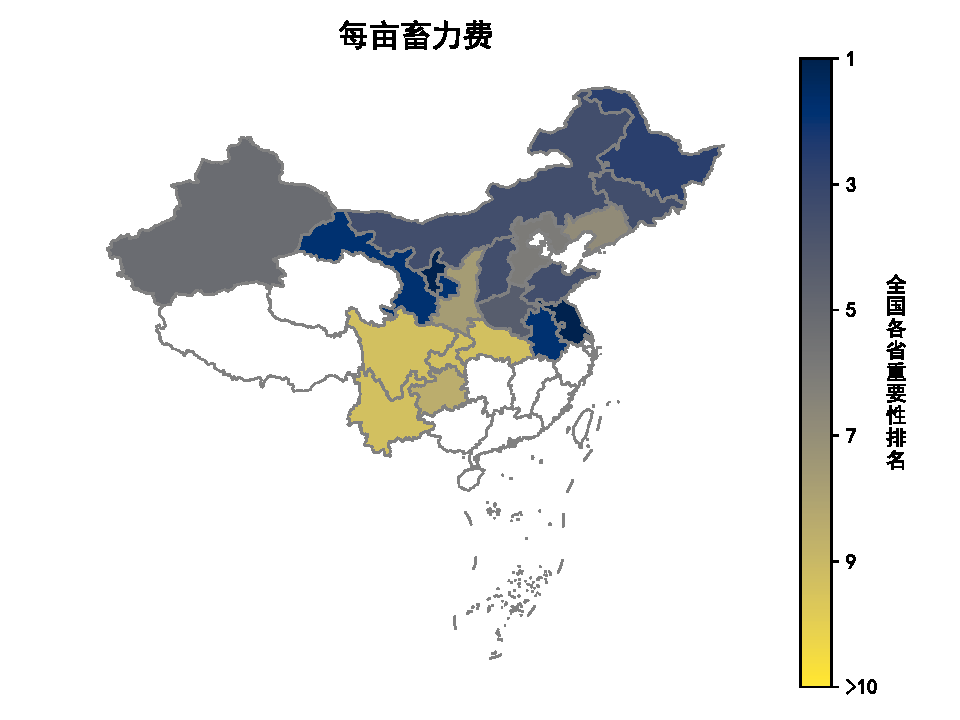
\includegraphics[width=\linewidth]{figs/cost_AniPower.pdf}
%     \caption{畜力费}
%     \label{fig:cost_AniPower}
%   \end{minipage}
%   \hfill
%   \begin{minipage}[t]{0.49\linewidth}
%     \centering
%     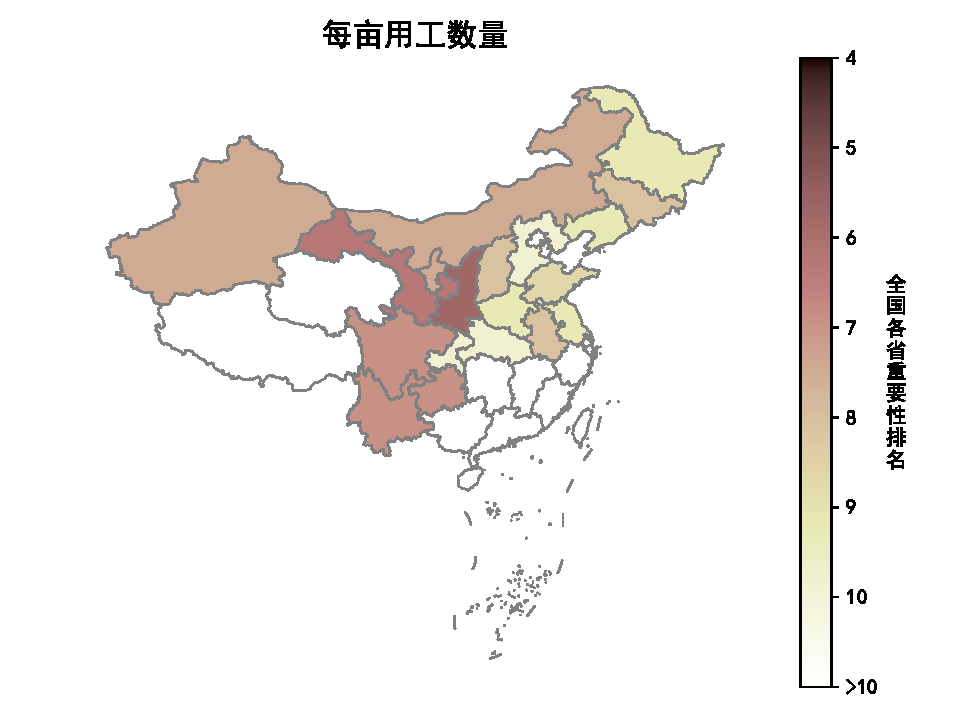
\includegraphics[width=\linewidth]{figs/cost_employ.pdf}
%     \caption{用工数}
%     \label{fig:cost_employ}
%   \end{minipage}\\[1em]
%   \begin{minipage}[t]{0.49\linewidth}
%     \centering
%     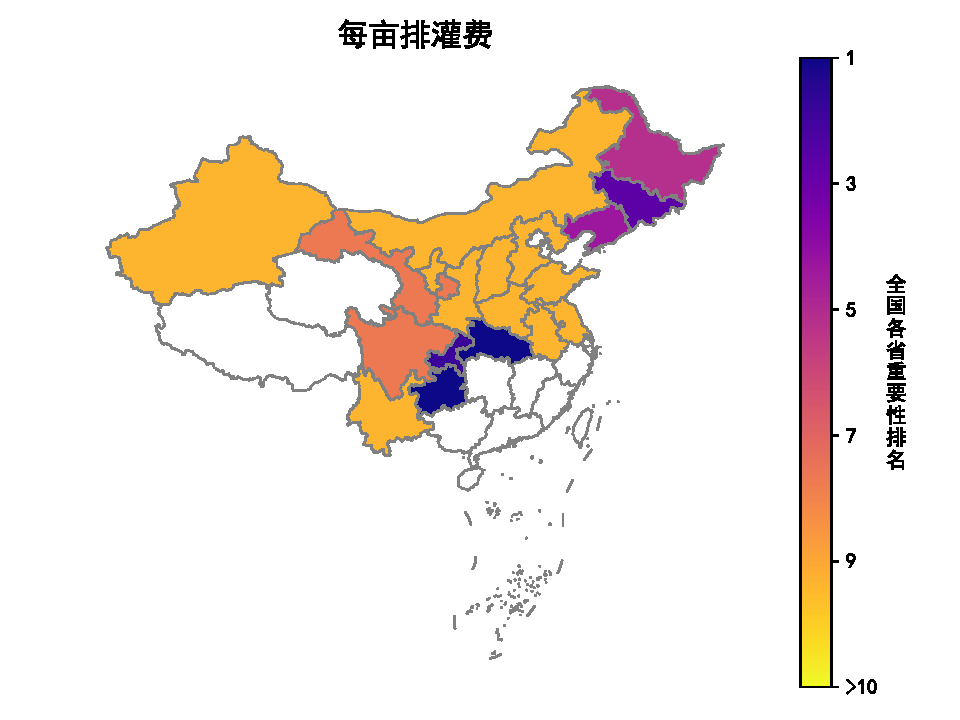
\includegraphics[width=\linewidth]{figs/cost_irrig.pdf}
%     \caption{排灌费}
%     \label{fig:cost_irrig}
%   \end{minipage}
%   \hfill
%   \begin{minipage}[t]{0.49\linewidth}
%     \centering
%     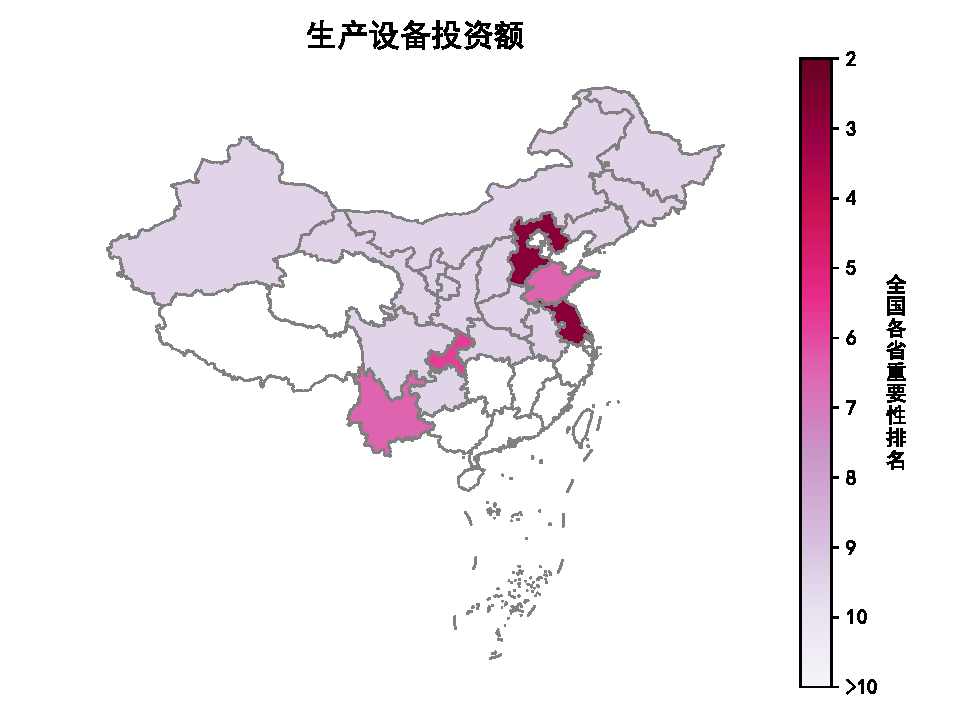
\includegraphics[width=\linewidth]{figs/rural_investment.pdf}
%     \caption{投资额}
%     \label{fig:rural_investment}
%   \end{minipage}
%   \caption{农资投入情况}
%   \label{fig:cost}
% \end{figure}

% 对于生产中投入的农资情况,在大多数省份中并不作为主要影响因素,只在少数省份中占主要影响因素。\ref{fig:cost}展示了相对最重要的4个因素作为分析对象,其余解释变量对玉米产量的影响重要性并不明显。

% \subsubsection{每亩畜力费}
% 每亩畜力费是一个综合的指标,涵盖了使用牲畜、畜力机械以及与其相关的各种费用。这个指标可以帮助了解在农业生产中使用畜力机械和牲畜所需的实际成本,进而对农业生产的投入和效益进行合理的分析。

% 一个地区的畜力费越高代表着其农业生产成本越高,而每亩畜力费在作物产量影响因素中越重要代表着在农业生产活动受到畜力费变化的影响较大,说明农业生产受到生产成本变化较严重。

% 由\ref{fig:cost_AniPower}可以看出,每亩畜力费在全国北方的重要性要远高于南方,考虑到北方地区的气候和土地条件相对于南方地区而言更加干旱,土地更加贫瘠,生产成本较高,因而在统筹农业生产规划的过程中需要注意我国南北方间生产成本的差异。

% \subsubsection{每亩用工数量}

% 每亩用工数量代表的是农业生产中的人工生产成本与人工生产效率,代表着农业生产的劳动力市场情况与农业机械化程度。由\ref{fig:cost_employ}可以明显看出,东部沿海地区普遍重要度较低,西部内陆地区重要度较高,说明由于我国东西部土地类型、气候条件、农业生产方式、农业机械化水平的不同,进而使得东部农业生产人工生产需求较低,西部相对较高。在西部地区农业劳动力的充足程度较低,而东部地区农业劳动力充足程度较高,农村劳动力市场在不同地区间产生了较大差异。

% 因此针对每亩用工数量对玉米产量的影响,应充分考虑地区间劳动力市场的差异,尽量减少我国东西部农村生产水平与生产成本的差异,可以通过推广农业机械化、提高农村生产条件、降低用工成本等减少每亩用工数量对玉米产量的限制,提高生产效率,从而提高玉米产量。

% \subsubsection{每亩排灌费}
% 每亩排灌费是指在农业生产中为了灌溉或排水而支出的费用。灌溉条件的好坏对产量有着重要的影响,同时排灌条件的建设与维护也需要耗费相应的资金与资源。

% 由\ref{fig:cost_irrig}可以看出,由于贵州、湖北、重庆等地区由于地形复杂气候湿润,对灌溉需求较大,灌排设施的建设难度较大,排灌系统建设费用相对较高,使得每亩排灌费对农业生产的影响程度较高。同时由\ref{fig:hazard_drought}中洪涝灾对玉米产量重要程度可得,贵州、湖北、重庆三省的玉米产量受到旱灾影响较为严重,这也间接说明了在这些省份排灌设备对而对于东北三省,气候较为寒冷,灌溉水源主要依靠人工补充,灌排系统对于低温和冻害等的应对需求较高,因此需要较高的排灌费用来保证农田的灌溉和排水,所以每亩排灌费对玉米产量的影响也更大。其他地区因地形或自然环境因素,对排灌需求不大或排灌设施已然完善,每亩排灌费对其玉米产量的影响便相对不特别重要。\cite{zhu2022investigating}

% 根据每亩排灌费对不同省份玉米产量的影响,可以得出排灌设施对农作物产量的重要性。对于受到排灌影响较大的省份,政府应该加大对这些地区的排灌设施建设和维护力度,提高排灌设施的效率与覆盖面积。对于受到排灌费影响较小的地区,也应加强设施的完善与维护,同时应鼓励农民使用节水灌溉技术,尽可能降低排灌成本与节约用水量。

% \subsubsection{生产设备投资额}

% 生产设备投资额是指在农业生产中用于购买和维护各种生产设备的资金支出,如农机具、灌溉设备等。在玉米产量影响因素中,生产设备投资额反映了农村在农业生产中采用现代化生产手段的程度和投入程度。\ref{fig:rural_investment}展示了生产设备投资额对各省玉米产量的影响重要程度。

% 农村生产设备投资额对玉米产量的影响主要与机械化水平、种植方式、技术水平等因素相关。河北、江苏等地区经济发达,农业机械化水平高,技术水平较高,因此农村生产设备投资额对其影响最大。而在其余一些影响不大的地区,可能由于农业现代化程度相对较低,生产设备投资对当地玉米产量提高的潜力仍未被充分发挥。

% 因此,政府还需加大对农村生产设备的投入,促进现代农业的发展,加大农业现代化建设力度,提高农业机械化水平和农业生产自动化程度。同时根据不同地区的实际情况,合理规划农村生产设备的投资方向和数量,确保投入有序和合理。最后还要加强对农业生产设备的研发和技术创新,推广新型农业机械和设备,提高农业生产效率和质量。

% 每亩修理维护费主要反映了农业机械设备的使用情况和维护保养水平。如果农业机械设备使用频率高、年限长、维护保养不及时,就会导致每亩修理维护费增加。

% 由\ref{fig:rural_investment}可以看出,对于沿海地区和川渝地区等发达地区,农业机械设备的使用情况和维护保养水平相对较高,因此每亩修理维护费对玉米产量的影响较低。而对于云南、内蒙古、河南内陆且对农业机械依赖度较大的省份,由于地理位置和自然环境等因素的影响,农业机械设备的使用情况和维护保养水平可能较低,所以每亩修理维护费对玉米产量的影响较大。

% 针对这一结果,我们需要在制定政策时重视农业机械设备的使用和维护保养,促进农业机械化水平的提高,降低每亩修理维护费用,从而提高玉米产量和农民收益。同时,也需要注意发达地区与欠发达地区的差异,有针对性地制定政策,促进农业机械化的均衡发展。

\section{粮食安全结论}
针对以上由基于属性重要度的模糊粗糙集属性约简算法得到的结果及分析,可以得到针对玉米生产及粮食安全的结论如下:
\subsection{结论}
\begin{enumerate}
  \item 磷肥与钾肥主要对个别集中的省份的影响较大。磷肥主要对我国内蒙古、黑龙江、宁夏、辽宁、山西等北部省份影响较大;钾肥主要对安徽、山西、湖北、重庆等中西部省份影响较大。内蒙古与山西同时受到磷肥与钾肥影响较大。
  \item 农业生产中的成本投入也是影响玉米产量的主要因素。每亩农膜用量对我国山东、河南、陕西、江苏、辽宁、吉林等省份的玉米生长影响较大;每亩人工成本则对我国四川、河北、江苏、陕西等省份的玉米生产影响较为显著。
  \item 水分在玉米的生长过程中有着重要的影响。除涝面积对于我国新疆、内蒙古、河北、山西等省份的玉米产量有着很大的影响;农用水泵则对我国黑龙江、宁夏、陕西、山东、云南等省份的玉米生产有着较大的影响。
  \item 机械化建设情况代表着农业生产现代化程度。节水灌溉类机械对我国云南、湖北、辽宁、宁夏等省份的玉米生产有着较大的影响;每亩修理维护费用对我国甘肃、宁夏、山西、新疆等省份有着不同程度的影响。
\end{enumerate}
\subsection{建议}
\begin{enumerate}
  \item 对于化肥施用量,在农业生产中需要因地制宜选择适合当地气候条件和土壤类型的肥料,根据不同地区的土壤养分特点和需求,科学施用磷肥和钾肥。对于受到磷肥钾肥影响较大的省份,建议农民在种植前进行土壤测试和养分评估,了解土壤中磷和钾的含量,以制定合理的施肥方案。并在不同的生长期注意合理施用磷肥和钾肥,避免过量或不足的施肥。同时政府还可以加强农业技术支持和培训,提高农民的施肥技术水平和肥料管理意识,以促进粮食安全和农业可持续发展。
  \item 对于成本投入情况,可以在重点地区积极推广农膜的合理使用和管理,并加强对农民的农业技术支持与培训,提高其农膜利用技术和人工成本控制管理的能力,注意农膜的回收和处理,减少对环境的负面影响。同时对于人工成本较高的省份政府还应推广机械化的建设与发展,利用现代农业机械和技术减少人工劳动,提高劳动生产率,合理安排劳动力的使用,减少玉米生产对人工劳动力的依赖。
  \item 对于排灌建设情况,在除涝面积重要性较高的省份,建议加强防涝工程建设和排水系统的改善,增加除涝面积,修建排水渠道和水利设施,以减少涝灾对玉米生长的不利影响。在农用水泵重要性较高的省份,可以加强对灌溉水资源的管理和技术支持,推广高效节水灌溉技术,合理安排灌溉计划,利用农用水泵提高灌溉水的利用效率。同时,还应加强气象监测和灾害预警,及时采取应对措施,减少自然灾害造成的损失。
  \item 对于机械化建设情况,在节水灌溉类机械重要性较高的省份,应加大对节水灌溉技术的推广和应用。引导农民采用滴灌、喷灌等高效灌溉方式,合理安排灌溉时间和水量,提高灌溉效率,增加玉米产量。在每亩修理与维护费重要性较高的省份,建议加强设备维护与管理,加强农业技术支持和培训,提高农民的技术水平和管理能力。通过培训农民了解最新的节水灌溉技术和设备维护方法,帮助他们更好地应用于实际生产中,提高玉米产量和质量。
\end{enumerate}


%%% Local Variables: 
%%% mode: latex
%%% TeX-master: "../main.tex"
%%% End:
